\documentclass[conference]{IEEEtran}
\usepackage{cite}
\usepackage{amsmath,amssymb,amsfonts}
\usepackage{graphicx}
\usepackage{booktabs}
\usepackage{tabularx}
\usepackage{tikz}
\usetikzlibrary{positioning, arrows.meta}

\begin{document}

\title{Optiguard}

\author{\IEEEauthorblockN{1\textsuperscript{st} Kuro Narendra Maheswara}
\IEEEauthorblockA{\textit{dept. name of organization (of Aff.)} \\
\textit{name of organization (of Aff.)}\\
City, Country \\
email address or ORCID}
\and
\IEEEauthorblockN{2\textsuperscript{nd} Jeljel Wirayudha Pratama Belanegara}
\IEEEauthorblockA{\textit{dept. name of organization (of Aff.)} \\
\textit{name of organization (of Aff.)}\\
City, Country \\
email address or ORCID}
\and
\IEEEauthorblockN{3\textsuperscript{rd} Chiko Bagaskara Adiwijaya}
\IEEEauthorblockA{\textit{dept. name of organization (of Aff.)} \\
\textit{name of organization (of Aff.)}\\
City, Country \\
email address or ORCID}
\and
\IEEEauthorblockN{4\textsuperscript{th} Michi}
\IEEEauthorblockA{\textit{dept. name of organization (of Aff.)} \\
\textit{name of organization (of Aff.)}\\
City, Country \\
email address or ORCID}
\and
\IEEEauthorblockN{5\textsuperscript{th} Rocky}
\IEEEauthorblockA{\textit{dept. name of organization (of Aff.)} \\
\textit{name of organization (of Aff.)}\\
City, Country \\
email address or ORCID}
\and
\IEEEauthorblockN{6\textsuperscript{th} Piko}
\IEEEauthorblockA{\textit{dept. name of organization (of Aff.)} \\
\textit{name of organization (of Aff.)}\\
City, Country \\
email address or ORCID}
}

\maketitle


\begin{abstract}
Placeholder abstract text.
\end{abstract}

\begin{IEEEkeywords}
VLM, surveillance, LoRA, DoRA
\end{IEEEkeywords}



\section{Introduction}
Vision impairment is one of the health problems experienced by many people around the world. It is estimated that more than 2.2 billion people worldwide have vision impairment, and at least 1 billion of them have vision impairments that are actually preventable or have not been adequately treated. Some of the diseases that can cause vision loss or even blindness are cataracts, diabetic retinopathy, and glaucoma \cite{WHO2023Blindness}. About 15.2 million people experience blindness due to cataracts, or about 45\% of all global blindness cases. In addition, cataracts are also the second largest cause of moderate to severe visual impairment, experienced by around 78.8 million people \cite{GBD2024Cataract}. Meanwhile, diabetic retinopathy continues to increase as the number of people with diabetes mellitus increases, with around 20\%–35\% of diabetics estimated to have diabetic retinopathy \cite{Pan2025DR}. The number of cases is projected to reach 129.84 million by 2030 and 160.50 million by 2045 \cite{Pan2025DR}. Glaucoma, as the leading cause of irreversible blindness in the world, is estimated to affect around 76 million people in 2020 and is projected to increase to 111.8 million people by 2040, with Asia and Africa being the most affected regions \cite{Vania2024Glaucoma}. These epidemiological facts underscore the urgency of developing accurate, affordable, and scalable early detection systems, particularly in low- and middle-income countries that face limited access to ophthalmological personnel.
\begin{figure*}[t]
    \centering
    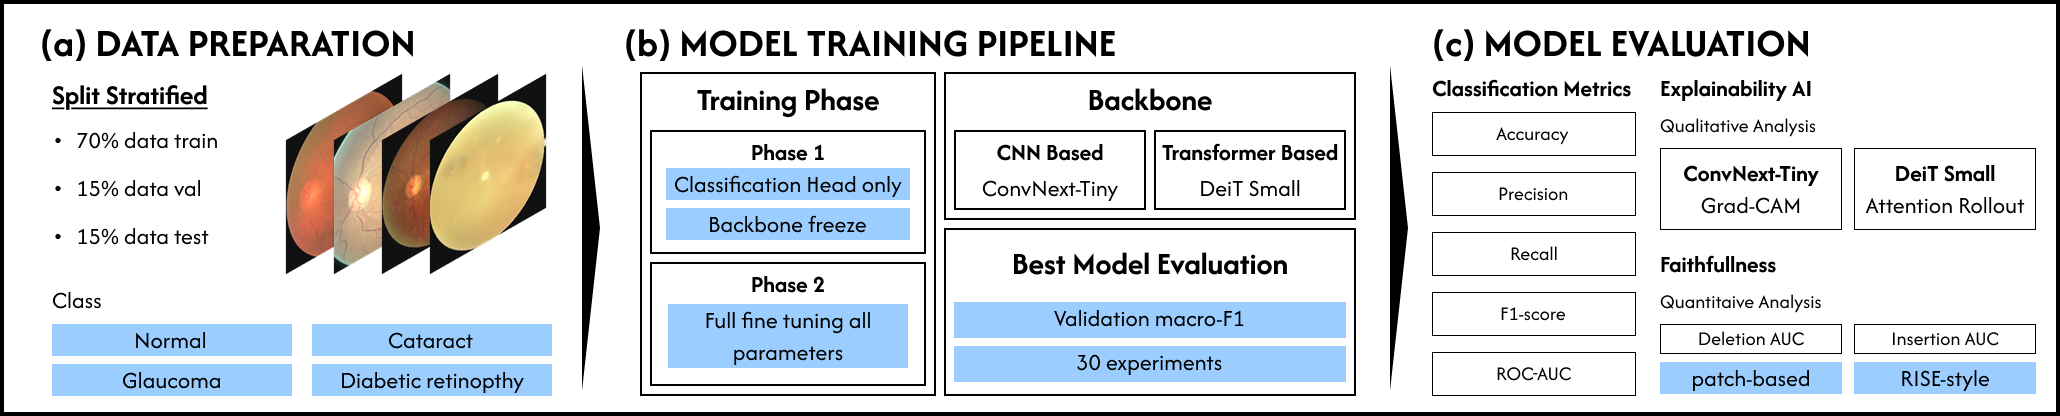
\includegraphics[width=\textwidth]{figures/methodology_version1}
    \caption{Overview of the research methodology.}
    \label{fig:methodology_overview}
\end{figure*}

To answer this need, a deep learning-based approach have been widely used in medical image analysis because it is able to extract features automatically from fundus images and other ophthalmological images without the need for manual feature extraction processes \cite{Elkholy2024OCT}. The development of deep learning architecture presents two main approaches, namely Convolutional Neural Network (CNNs) and Vision Transformer (ViTs). One of the latest CNN architectures is ConvNeXt, which was developed by adopting some of the design principles of the Vision Transformer so that it can improve accuracy while maintaining CNN efficiency \cite{Liu2022}. On the other hand, the Vision Transformer (ViT) uses a self-attention mechanism to learn the relationships between parts of the image. One of the developments is the Data-efficient Image Transformer (DeiT), which allows models to be trained effectively using smaller datasets with lower computational requirements through knowledge distillation techniques \cite{touvron2021trainingdataefficientimagetransformers}.

Although deep learning models have very high classification accuracy, they often suffer from a black-box limitation. This means that the model can provide accurate predictions, but the process behind its decision-making is not transparent and is difficult for humans to understand \cite{Gomez2022Saliency}. Therefore, Explainable Artificial Intelligence (XAI) technology is used to visualize the reasoning behind the model's predictions. For models that use CNN architecture such as ConvNeXt, the Grad-CAM method is typically used to create a heatmap that highlights the most important areas of the image. Meanwhile, in Transformer architectures such as DeiT, the method used is Attention Rollout or Gradient Attention Rollout. This method works by collecting the attention weights of each layer of the model to see which parts of the image the model is most focused on \cite{Cho2025GMAR}. The different internal mechanisms of these two models mean that the quality of the resulting visualizations is not directly comparable. The main problem is that current deep learning evaluations in the medical field mostly stop at accuracy comparison. To quantitatively measure how faithful these visualizations are, specific metrics are required. Deletion and insertion metrics that use Area Under Curve (AUC) values are often used as the standard of measurement. These metrics work by gradually hiding or showing parts of the image according to their importance, and then seeing how much the model's confidence level in its predictions changes \cite{Gomez2022Saliency}.  

Based on the problems that have been described, the focus of this research is formulated into two main analytical scopes. The first focus is on a comparative evaluation of the classification performance between the ConvNeXt and DeiT architectures on a dataset of four classes of eye diseases (cataracts, diabetic retinopathy, glaucoma, and normal) using accuracy, precision, recall, and F1-score metrics. The second focus is a comparative analysis of the quality of visual explanations, particularly at the level of faithfulness of heatmap representation, between the Grad-CAM method in the ConvNeXt model and the Attention Rollout in the DeiT model, which is quantitatively evaluated through deletion AUC and insertion AUC measurements.

To address these problems, this research presents two main contributions. Theoretically, this study enriches the academic literature related to the comparative interpretability between modern CNN (ConvNeXt) and Vision Transformer (DeiT) architectures that are specialized in the domain of ophthalmological medical imaging. previous research that rarely explored the comparison of models in depth based on the faithfulness parameters of XAI visualizations, instead of relying solely on accuracy metrics. Meanwhile, practically, this study provides an empirical evidence-based guideline for clinical practitioners and engineers in determining the combination of XAI architecture and methods that best suits the needs of operational systems. For example, the results of this research can be used as a direct reference in choosing the most recommended architecture when a diagnostic system requires a heatmap localization that is highly aligned with the model's decision-making basis.

\section{Related Work}
\subsection{Deep Learning-Based Eye Disease Classification}

Deep learning-based eye disease classification using fundus images has attracted significant research attention in recent years. The Eye Disease Classification dataset \cite{dataset} is one of the publicly available datasets frequently used for benchmarking multiclass eye disease classification models. The characteristics of the dataset are presented in Table~\ref{tab:dataset}.

\begin{table}[htbp]
\caption{Distribution of Eye Disease Classification Dataset}
\label{tab:dataset}
\centering
\begin{tabular}{lcc}
\toprule
\textbf{Class} & \textbf{Number of Images} & \textbf{Percentage (\%)} \\
\midrule
Cataract & 1,038 & 24.62 \\
Diabetic Retinopathy & 1,098 & 26.04 \\
Glaucoma & 1,007 & 23.88 \\
Normal & 1,074 & 25.47 \\
\midrule
\textbf{Total} & \textbf{4,217} & \textbf{100.00} \\
\bottomrule
\end{tabular}
\end{table}

Dataset characteristics are relatively consistent across studies, comprising 4,217 fundus images categorized into four classes: cataract, diabetic retinopathy, glaucoma, and normal eyes \cite{erdas2024,jibon2025}. Although the dataset is relatively balanced, glaucoma represents the minority class, which motivates the use of data augmentation techniques during preprocessing.

The dataset has been utilized in several studies to evaluate the performance of deep learning models. A comparative study involving DenseNet, EfficientNet, Xception, VGG, and ResNet was conducted in \cite{erdas2024}. Among these architectures, EfficientNet achieved the highest accuracy of 87.84\%. Subsequently, transfer learning with EfficientNet-B3 combined with data augmentation and cosine annealing learning rate scheduling was proposed in \cite{alsohemi2025}, resulting in an improved accuracy of 95.12\%.

A transfer learning framework named TL-MED was introduced in \cite{jibon2025}, where five CNN-based architectures and an ensemble model were evaluated. DenseNet169 achieved the highest individual accuracy of 96\%. In another study, AlexNet, EfficientNet-B0, EfficientNet-B7, and a custom CNN architecture were compared \cite{elkenawy2026}. AlexNet demonstrated the best performance with an accuracy of 93.65\%, and the study further employed SHAP-based interpretability analysis to identify clinically relevant image regions. Beyond SHAP, gradient-based visualization techniques such as Grad-CAM \cite{Selvaraju2017} have also been widely adopted in fundus image classification studies to highlight discriminative regions contributing to the model's prediction, providing a complementary means of interpreting CNN-based decisions.

Based on these studies, existing research on this dataset primarily focuses on conventional CNN architectures and their variants, including VGG, ResNet, DenseNet, EfficientNet, and AlexNet. In contrast, investigations involving modern CNN architectures such as ConvNeXt and transformer-based architectures such as DeiT remain limited. This research gap motivates the comparative analysis conducted in this study.

\subsection{ConvNeXt and DeiT Architectures for Image Analysis}

As representative architectures of modern convolutional networks and vision transformers, ConvNeXt and DeiT have demonstrated promising performance across various image classification tasks. ConvNeXt was introduced in \cite{Liu2022} as a modernization of the ResNet architecture by incorporating several design principles inspired by Vision Transformers, including patchify stems, depthwise convolutions, inverted bottlenecks, larger kernel sizes, and simplified normalization and activation layers.

On the other hand, DeiT (Data-efficient Image Transformer) was proposed in \cite{touvron2021trainingdataefficientimagetransformers} as an extension of the original Vision Transformer architecture \cite{dosovitskiy2021imageworth16x16words}. DeiT introduces a knowledge distillation strategy that enables transformer models to be trained effectively on relatively smaller datasets while maintaining competitive performance.

Several comparative studies have investigated the strengths and limitations of CNN and Vision Transformer architectures in image analysis tasks. A literature review presented in \cite{mauricio2023} concluded that CNNs benefit from strong inductive biases and superior data efficiency, whereas Vision Transformers are more effective at capturing global contextual information but generally require larger datasets and greater computational resources.

In the specific domain of fundus image analysis, a comparative study between CNN-based architectures, including ConvNeXt, and transformer-based models was conducted in \cite{alayon2023}. The results showed that the transformer-based CaiT architecture achieved the highest AUC of 0.979, although the performance gap between the best CNN and transformer models was relatively small. Similar findings were reported in \cite{hwang2023}, where Vision Transformer models achieved non-inferior or superior performance compared with CNNs on five out of six glaucoma datasets.

Overall, these findings suggest that the relative advantages of modern CNN architectures such as ConvNeXt and transformer-based architectures such as DeiT depend heavily on dataset characteristics and training strategies. Therefore, no clear consensus has emerged regarding the superiority of either approach. This motivates a direct comparison between ConvNeXt and DeiT for multiclass eye disease classification using the Eye Disease Classification dataset.
\section{Methodology}

\subsection{Model Architecture}

\subsubsection{ConvNeXt}

ConvNeXt is a modern convolutional neural network (CNN) architecture inspired by Vision Transformers (ViTs). It modernizes standard convolutional operations without relying on self-attention mechanisms. Specifically, ConvNeXt redesigns the standard ResNet architecture by adopting $7 \times 7$ depthwise convolution to enlarge the receptive field, using inverted bottleneck blocks, replacing Batch Normalization with LayerNorm, and replacing Rectified Linear Unit (ReLU) with GELU to improve optimization stability during transfer learning \cite{Liu2022}. These architectural refinements enhance feature representation without sacrificing the computational advantages of convolution-based networks. Fig.~\ref{fig:convnext_block} illustrates the internal structural flow of a ConvNeXt block.

\begin{figure}[htbp]
    \centering
    \resizebox{\columnwidth}{!}{
        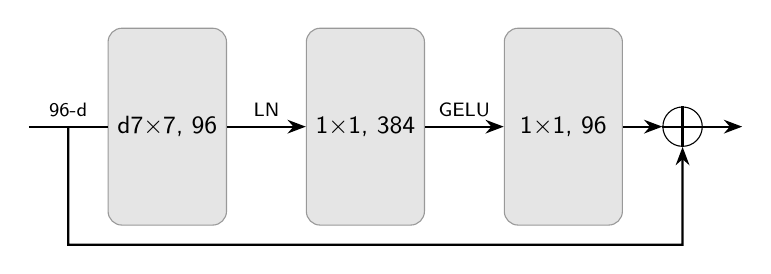
\begin{tikzpicture}[
            block/.style={
                rectangle,
                draw=gray!80,
                fill=gray!20,
                minimum width=1.5cm,
                minimum height=2.5cm,
                rounded corners=5pt,
                align=center,
                font=\small\sffamily
            },
            arrow/.style={
                ->,
                >=Stealth,
                thick
            },
            add/.style={
                circle,
                draw,
                minimum size=0.5cm,
                inner sep=0pt
            }
        ]
            \coordinate (input) at (0,0);

            \node [block, right=1cm of input] (b1) {d7$\times$7, 96};
            \node [block, right=1cm of b1] (b2) {1$\times$1, 384};
            \node [block, right=1cm of b2] (b3) {1$\times$1, 96};
            \node [add, right=0.5cm of b3] (plus) {};

            \draw[thick] (plus.north) -- (plus.south);
            \draw[thick] (plus.west) -- (plus.east);

            \coordinate [right=0.5cm of plus] (output);

            \coordinate (split) at (0.5,0);

            \draw [thick] (input) -- (b1.west) node[midway, above, font=\scriptsize\sffamily] {96-d};
            \draw [arrow] (b1.east) -- (b2.west) node[midway, above, font=\scriptsize\sffamily] {LN};
            \draw [arrow] (b2.east) -- (b3.west) node[midway, above, font=\scriptsize\sffamily] {GELU};
            \draw [arrow] (b3.east) -- (plus.west);
            \draw [arrow] (plus.east) -- (output);

            \draw [arrow] (split) -- (0.5,-1.5)
                                -- ([yshift=-1.5cm]plus.center)
                                -- (plus.south);

        \end{tikzpicture}
    }
    \caption{ConvNeXt Block Architecture.}
    \label{fig:convnext_block}
\end{figure}

To evaluate its real-world efficacy, a recent large-scale study compared ConvNeXt, RegNet, and ResNet across $22$ publicly available retinal fundus datasets \cite{Chopowiec2023}. This benchmark comprised more than $125,000$ images spanning normal cases, diabetic retinopathy, glaucoma, and age-related macular degeneration to construct a clinically representative screening model. Among the tested architectures, ConvNeXt-Tiny achieved the best overall performance across most evaluation metrics, obtaining an overall accuracy of $80.46 \pm 1.48\%$. It demonstrated particularly high disease recognition accuracy for glaucoma ($97.20\%$), age-related macular degeneration ($98.14\%$), and diabetic retinopathy ($80.66\%$) These findings demonstrated ConvNeXt-Tiny's reliability for retinal disease classification while maintaining a relatively lightweight architecture, making it highly suitable for transfer learning on moderately sized retinal fundus datasets.

\subsubsection{DeiT}

Standard Vision Transformers (ViTs) rely primarily on self-attention mechanisms to capture long-range dependencies across an entire image and generally require extremely large-scale pretraining datasets to achieve competitive performance \cite{dosovitskiy2021imageworth16x16words}. To overcome these substantial data requirements while preserving the advantages of transformer-based architectures, Data-efficient Image Transformers (DeiT) were proposed \cite{touvron2021trainingdataefficientimagetransformers}.
DeiT introduces a dedicated distillation token into the architecture, which is appended alongside the class token and patch embeddings as illustrated in Fig.~\ref{fig:deit_block}. During training, this token interacts with the patch tokens via self-attention to learn complementary features from a robust, pretrained teacher model (typically a CNN). This mechanism significantly improves classification accuracy, particularly for smaller transformer models, while maintaining computational efficiency.

\begin{figure}
    \centering
    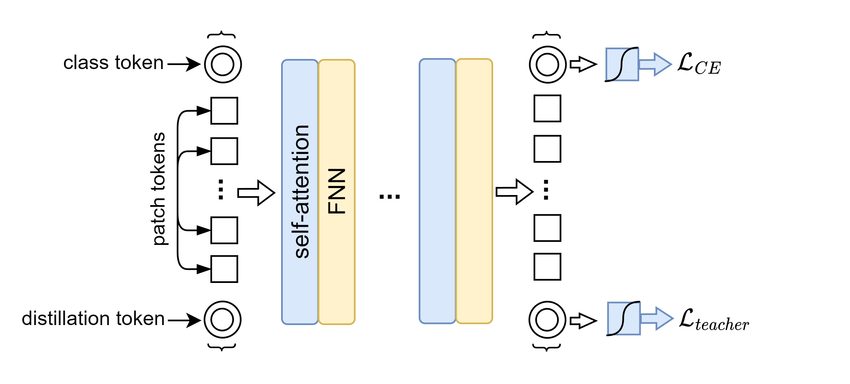
\includegraphics[width=0.45\textwidth]{figures/DeiT-main-architecture.png}
    \caption{DeiT Block Architecture}
    \label{fig:deit_block}
\end{figure}

The data-efficient design of DeiT makes it particularly suitable for medical image analysis, where large annotated datasets are often unavailable and training standard ViTs from scratch is difficult. A recent study incorporated DeiT as one of the transformer-based feature extractors in a hybrid framework for multi-class eye disease classification, demonstrating that combining DeiT with machine learning classifiers contributed to a stacking model that achieved $97.163\%$ classification accuracy on a benchmark retinal dataset \cite{AlMohimeed2025}. These findings indicate that transformer-based models can be effectively applied to retinal disease classification when equipped with efficient training or feature extraction strategies. Therefore, DeiT is suitable for transfer learning as a representative data-efficient Vision Transformer for a moderately sized retinal fundus datasets.

\subsubsection{Hyperparameter \& Model Selection}

Model parameters refer to the network weights that are automatically learned through backpropagation, whereas hyperparameters are predefined before or during training to control the optimization process, regularization, and learning schedule \cite{Bengio2000}. During transfer learning and fine-tuning, commonly configured hyperparameters include the learning rate, batch size, weight decay, optimizer, learning-rate scheduler, data augmentation strategy, number of training epochs, and early stopping criterion. Hyperparameter optimization can be performed using several strategies, including grid search, random search, and manual tuning. Out of those three, random search is generally more efficient than grid search because only a small subset of hyperparameters typically has a significant influence on model performance, and the importance of individual hyperparameters may vary across different datasets \cite{JMLR:v13:bergstra12a}.

To ensure an unbiased evaluation, the dataset is divided into training, validation, and testing subsets. The training set is used to optimize the model parameters, whereas the validation set is exclusively used to select the best hyperparameter configuration and training scenario \cite{Reyes2024}. The test set is used solely for the final performance evaluation and is not involved in any stage of model selection or hyperparameter optimization \cite{Jiang2021}. This separation prevents information leakage and optimistic bias, resulting in a more reliable estimation of the model's generalization capability.

\subsection{Explainable AI (XAI) on Computer Vision}

\subsubsection{Grad-CAM}

For a target class $c$, Grad-CAM first backpropagates the class score $y^c$ with respect to each feature map $A^k$ in the final convolutional layer. The importance weight of the $k$-th feature map is obtained by applying global average pooling to the spatial gradients, which is defined as

\begin{equation}
\alpha_{k}^{c} = \frac{1}{Z} \sum_{i} \sum_{j} \frac{\partial y^{c}}{\partial A_{i,j}^{k}}
\label{eq:grad_cam_weights}
\end{equation}

where $Z$ denotes the total number of spatial locations in the feature map. The resulting weight $\alpha_k^c$ represents the contribution of feature map $A^k$ to the prediction of class $c$ \cite{Selvaraju2020}.

The class activation map is subsequently generated as a weighted combination of all feature maps,

\begin{equation}
    L_{Grad-CAM}^{c} = ReLU (\sum_{k} \alpha_{k}^{c} A^{k})
    \label{eq:grad_cam_activation_map}
\end{equation}

where the ReLU suppresses negative activations, preserving only features that positively influence the prediction of the target class \cite{Selvaraju2020}.

Although originally developed for CNNs, Grad-CAM has been successfully adapted to Vision Transformers. The method utilizes the patch token representations extracted from the final transformer encoder block, which are reshaped into a two-dimensional spatial grid before gradient computation. The spatial gradients are globally averaged to obtain token importance weights, followed by weighted aggregation and ReLU activation to produce the final saliency map \cite{Alhafdhi2026, Vanitha2025}.

Grad-CAM has been widely adopted in medical image analysis to verify whether deep learning models focus on clinically relevant anatomical structures or pathological lesions. As summarized in Table~\ref{tab:medical_gradcam_comparison}, Grad-CAM has demonstrated its effectiveness across multiple imaging modalities and deep learning architectures.

\begin{table}[htbp]
    \caption{Applications of Grad-CAM in Medical Image Analysis.}
    \label{tab:medical_gradcam_comparison}
    \centering
    \small
    \setlength{\tabcolsep}{4pt}
    \begin{tabularx}{\columnwidth}{>{\raggedright\arraybackslash}p{2.6cm} >{\raggedright\arraybackslash}p{2cm} >{\raggedright\arraybackslash}X}
        \toprule
        \textbf{Medical Domain} & \textbf{Architecture} & \textbf{Interpretability Outcome} \\
        \midrule
        Chest X-ray (TB) &
        ViT &
        Highlights diagnostically relevant pulmonary regions, enabling visualization of the model's focus during tuberculosis classification \cite{Vanitha2025}.\\
        \addlinespace

        Retinal disease &
        ResNet101-V2 &
        Emphasizes retinal abnormalities associated with glaucoma, diabetic retinopathy, and cataracts, improving multiclass model interpretability \cite{AbdEl-Ghany2025}.\\
        \addlinespace

        Thyroid ultrasound &
        Hybrid CNN--ViT &
        Produces clinically meaningful activation patterns that validate lesion localization and support prediction reliability \cite{Alhafdhi2026}.\\
        \bottomrule
    \end{tabularx}
\end{table}

\subsubsection{Attention Rollout}

Vision Transformers compute a self-attention matrix at every transformer layer, where each element represents the attention weight assigned from one token to another. Since each image patch is represented as a token, the attention matrix describes how information is exchanged among all image patches through the self-attention mechanism. Self-attention enables every token to interact with all other tokens, allowing the model to capture global contextual relationships, unlike convolutional neural networks that rely on local receptive fields \cite{dosovitskiy2021imageworth16x16words}.

However, the attention matrix from a single transformer layer only reflects the interaction at that particular layer and does not directly indicate the overall contribution of an input patch to the final prediction. To estimate how information propagates throughout the transformer, Attention Rollout recursively composes the attention matrices from consecutive layers. Consequently, the importance of each input patch is determined by the accumulated attention flow from the input layer to the final class token representation \cite{Abnar2020}.

The recursive formulation of Attention Rollout is expressed as

\begin{equation}
    \tilde{A}(l_{i}) = \begin{cases}
        {A}(l_{i}) \tilde{A}(l_{i-1})   & \text{if } i > j\\
        {A}(l_{i})                      & \text{if } i = j
    \end{cases}
    \label{attention_rollout_equation}
\end{equation}

where $A(l_i)$ denotes the attention matrix of the $i$-th transformer layer, while $\tilde{A}(l_i)$ represents the accumulated attention after recursively composing the attention matrices from previous layers. For image classification, the attention values corresponding to the class (CLS) token in the final rollout matrix are reshaped into the spatial arrangement of the input patches to generate the explanation heatmap \cite{Abnar2020}.

Compared with gradient-based explanation methods, Attention Rollout provides a global interpretation by tracing information flow through all transformer layers rather than relying on the gradients of a single layer. The resulting heatmaps tend to be more diffused and less spatially localized than those produced by Grad-CAM, because the explanation aggregates attention across multiple layers \cite{Cheng2025,Li2023}. A summary of the differences between Attention Rollout and Grad-CAM is presented in Table~\ref{tab:gradcam_rollout}.

\begin{table}[htbp]
    \caption{Comparison between Grad-CAM and Attention Rollout}
    \label{tab:gradcam_rollout}
    \centering
    \small
    \setlength{\tabcolsep}{6pt}
    \begin{tabularx}{\columnwidth}{>{\raggedright\arraybackslash}p{2.5cm} >{\raggedright\arraybackslash}X}
        \toprule
        \textbf{Method} & \textbf{Characteristics} \\
        \midrule
        Grad-CAM &
        Produces class-discriminative heatmaps using gradients from the last convolutional feature map. It provides relatively sharp and localized visual explanations but is primarily designed for CNNs. \\

        \addlinespace
        Attention Rollout &
        Propagates attention recursively across transformer layers to estimate the contribution of each input patch to the CLS token. It captures global contextual relationships but generally produces more diffuse heatmaps than Grad-CAM. \\
        \bottomrule
    \end{tabularx}
\end{table}

\subsection{Faithfulness Evaluation}

The quality of the generated saliency maps was quantitatively evaluated using the deletion and insertion Area Under the Curve (AUC) metrics. These metrics are both model-agnostic and explanation-agnostic because they assess explanation quality based solely on changes in the model prediction after perturbing the input image, regardless of the internal mechanism used to generate the explanation \cite{petsiuk2018riserandomizedinputsampling, Skliarov2025}. Deletion AUC measures whether the pixels identified as important by a saliency map are truly critical for the model prediction, while insertion AUC measures how effectively the highlighted regions restore the model prediction.

Deletion AUC starts by ranking all image pixels according to their importance values in the generated heatmap. Then, the most important pixels are then progressively removed or replaced with a predefined baseline while the confidence score of the target class is recorded after each steps \cite{petsiuk2018riserandomizedinputsampling}. The AUC is then calculated from plotting the resulting confidence values against the fraction of removed pixels, where a lower AUC indicates a more faithful explanation because the model confidence decreases rapidly when the truly relevant regions are removed \cite{Cheng2025}.

Insertion AUC starts with an uninformative baseline image and the most important pixels are gradually inserted according to their ranking in the saliency map \cite{petsiuk2018riserandomizedinputsampling}. The AUC is then calculated from plotting the prediction confidence against the fraction of inserted pixels, where a higher AUC indicates a more faithful explanation because the selected pixels rapidly recover the confidence of the target prediction \cite{Cheng2025}.

\section{Results}

This section presents the experimental results of the study, organized according to the two analytical scopes defined in Section~I: (1) the classification performance comparison between ConvNeXt-Tiny and DeiT-Small, and (2) the faithfulness comparison between Grad-CAM and Attention Rollout as measured by deletion and insertion AUC.

\subsection{Hyperparameter Selection}

Both ConvNeXt-Tiny and DeiT-Small were fine-tuned using a two-phase training scheme (linear-probe followed by full fine-tuning) under a grid search over learning rate and number of training epochs. For each architecture, the configuration achieving the highest validation macro-F1 was selected as the final model, following the model selection protocol described in Section~III-A. Table~\ref{tab:hyperparam_selection} summarizes the selected configuration for each architecture.

\begin{table}[htbp]
\caption{Selected Hyperparameter Configuration per Architecture}
\label{tab:hyperparam_selection}
\centering
\begin{tabular}{lcc}
\toprule
\textbf{Hyperparameter} & \textbf{ConvNeXt-Tiny} & \textbf{DeiT-Small} \\
\midrule
Linear probe learning rate & $1\times10^{-3}$ & $1\times10^{-3}$ \\
Full fine-tuning learning rate & $5\times10^{-5}$ & $1\times5^{-5}$ \\
Weight decay & $0.05$ & $0.05$ \\
Label smoothing & $0.1$ & $0.1$ \\
Linear probe epochs & 5 & 5 \\
Full fine-tuning epochs & 45 & 45 \\
Batch size & 32 & 32 \\
\bottomrule
\end{tabular}
\end{table}

The selected configuration for each architecture converged well before its configured epoch budget was exhausted (epoch 11 of 30 for ConvNeXt-Tiny, epoch 19 of 40 for DeiT-Small), consistent with the two-phase fine-tuning scheme reaching its best validation macro-F1 early in the full-fine-tuning phase. The full ranking of all $15$ grid-search combinations per architecture is available in the accompanying evaluation notebook (\texttt{eval.ipynb}).

\subsection{Classification Performance}

Table~\ref{tab:classification_performance} presents the test-set classification performance of both architectures, reported as overall accuracy and macro-averaged precision, recall, and F1-score. Diabetic retinopathy recall is reported separately, as it serves as the tie-breaker criterion for final model selection due to the higher clinical cost of false-negative diagnoses.

\begin{table}[htbp]
\caption{Test-Set Classification Performance}
\label{tab:classification_performance}
\centering
\begin{tabular}{lcc}
\toprule
\textbf{Metric} & \textbf{ConvNeXt-Tiny} & \textbf{DeiT-Small} \\
\midrule
Accuracy & 87.99\% & 87.99\% \\
Macro Precision & 87.91\% & 88.03\% \\
Macro Recall & 87.74\% & 87.77\% \\
Macro F1-score & 87.63\% & \textbf{87.74\%} \\
Macro ROC-AUC & \textbf{98.15\%} & 97.06\% \\
DR Recall (tie-breaker) & \textbf{99.39\%} & 95.76\% \\
\bottomrule
\end{tabular}
\end{table}

Table~\ref{tab:per_class_performance} further reports the per-class precision, recall, and F1-score for the winning model, providing a more detailed view of class-wise classification behavior, particularly for the minority glaucoma class.

\begin{table}[htbp]
\caption{Per-Class Performance of the Selected Model (DeiT-Small)}
\label{tab:per_class_performance}
\centering
\begin{tabular}{lccc}
\toprule
\textbf{Class} & \textbf{Precision} & \textbf{Recall} & \textbf{F1-score} \\
\midrule
Cataract & 93.46\% & 91.67\% & 92.56\% \\
Diabetic Retinopathy & 87.78\% & 95.76\% & 91.59\% \\
Glaucoma & 86.26\% & 74.83\% & 80.14\% \\
Normal & 84.62\% & 88.82\% & 86.67\% \\
\bottomrule
\end{tabular}
\end{table}

Based on the test-set macro-F1, DeiT-Small (87.74\%) marginally outperformed ConvNeXt-Tiny (87.63\%) -- a gap of only $0.11$ percentage points, small enough that the two architectures are effectively comparable in overall discriminative power. Since the macro-F1 values were not exactly tied, the diabetic retinopathy recall tie-breaker was not formally invoked; however, it is worth noting that ConvNeXt-Tiny attained a substantially higher DR recall ($99.39\%$ vs. $95.76\%$) and macro ROC-AUC ($98.15\%$ vs. $97.06\%$), a discrepancy discussed further in Section~IV-E. Per the strict macro-F1 ranking, DeiT-Small is treated as the best-performing architecture and is used as the subject of the per-class analysis above; both architectures' checkpoints are nonetheless carried forward into the explainability analysis in the following subsections, since faithfulness is compared architecture-to-architecture (Grad-CAM vs. Attention Rollout) rather than reduced to a single winner. Both models show the same qualitative weak point: glaucoma has the lowest recall of the four classes ($74.83\%$ for DeiT-Small), reflecting its status as the dataset's minority class (Table~\ref{tab:dataset}).

Fig.~\ref{fig:confusion_matrix} shows the row-normalized confusion matrix of the selected model (DeiT-Small) on the test set, confirming that glaucoma is most frequently confused with cataract and normal, while diabetic retinopathy and cataract are both classified with high recall.

\begin{figure}[htbp]
    \centering
    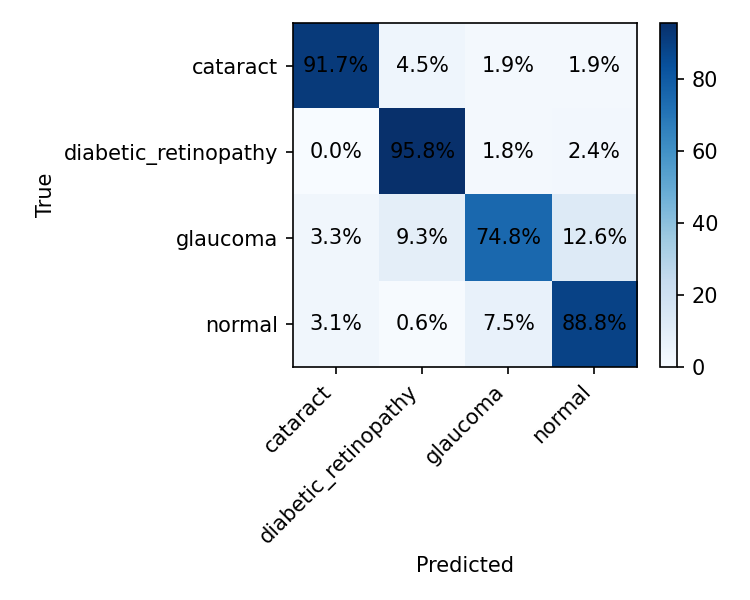
\includegraphics[width=0.45\textwidth]{figures/confusion_matrix.png}
    \caption{Normalized confusion matrix of the selected model (DeiT-Small) on the test set.}
    \label{fig:confusion_matrix}
\end{figure}

\subsection{Qualitative Explainability Results}

Fig.~\ref{fig:xai_qualitative} presents qualitative examples of Grad-CAM heatmaps generated from ConvNeXt-Tiny and Attention Rollout heatmaps generated from DeiT-Small on representative test images from each class. For glaucoma and diabetic retinopathy, both methods concentrate their highest activations tightly on the optic disc region -- the clinically relevant structure for assessing cupping in glaucoma and a common site of hemorrhages and exudates in diabetic retinopathy -- indicating that both models learned to attend to anatomically meaningful evidence rather than spurious background cues for these two classes. For the normal example, both methods likewise center on the optic disc and surrounding vasculature, consistent with this being the reference structure clinicians inspect first. Cataract is the weakest case for both methods: Grad-CAM activates a narrow vertical strip near the image border rather than a diffuse haze pattern (the actual visual signature of a cataract in a fundus photo), while Attention Rollout spreads its attention toward the image corners and edges outside the fundus circle. This is consistent with cataract's presentation as a global loss of image sharpness/contrast rather than a spatially localized lesion, which is inherently harder for patch-level saliency methods -- both CNN- and attention-based -- to localize. Attention Rollout's tendency to assign non-trivial weight to border/corner patches across multiple classes also matches its characterization in Section~III-B as producing more diffuse heatmaps than Grad-CAM.

\begin{figure*}[t]
    \centering
    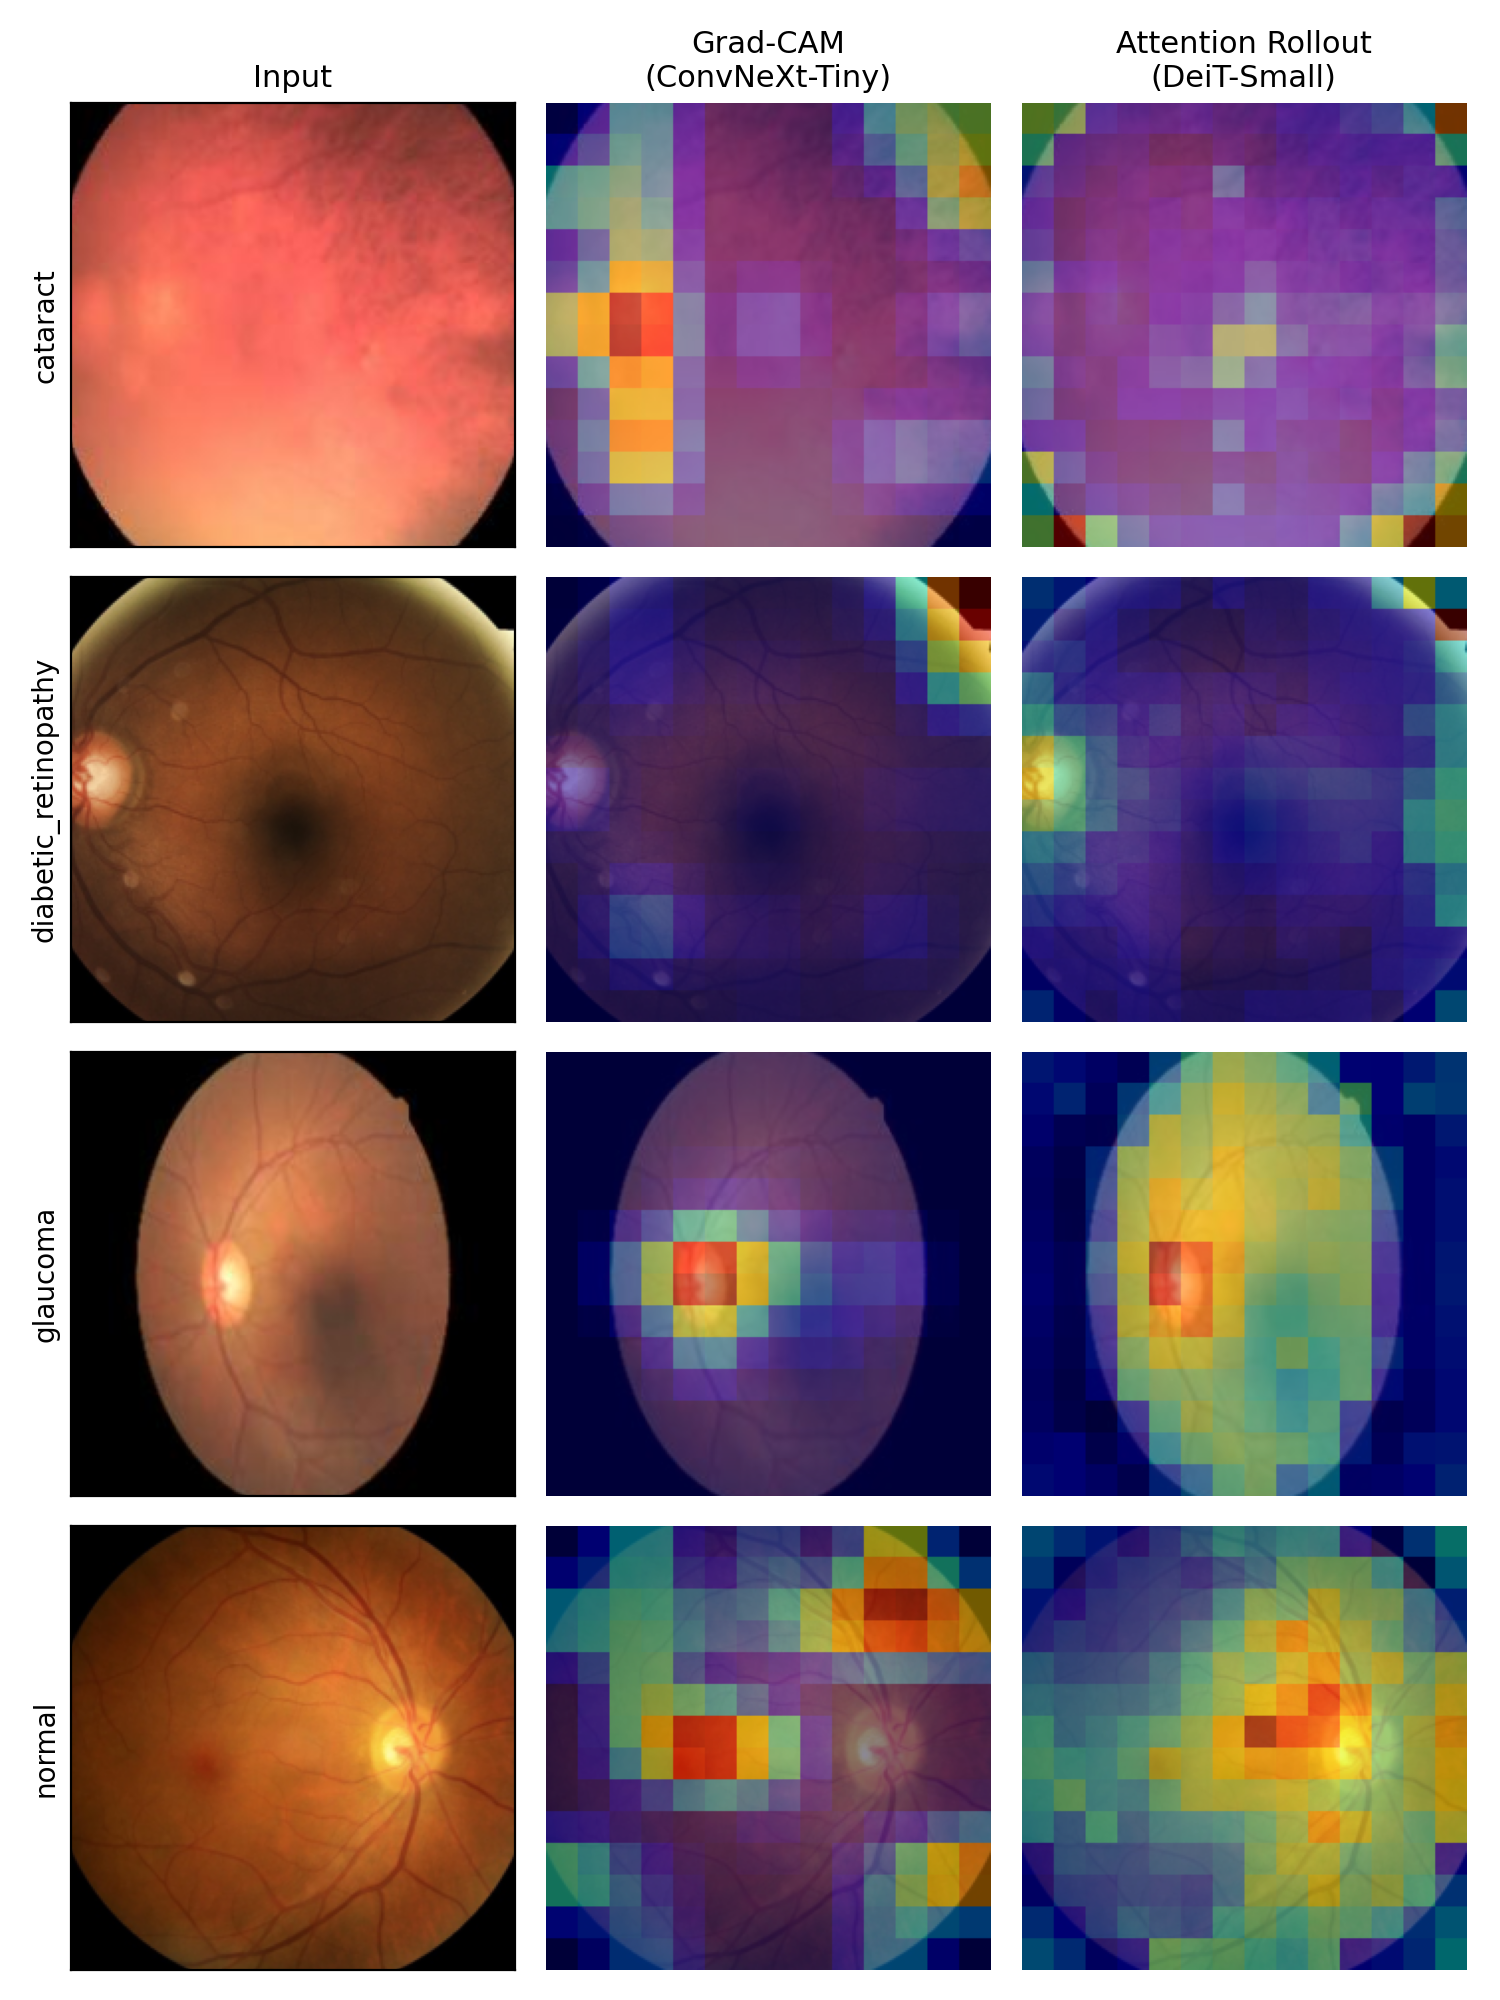
\includegraphics[width=\textwidth,height=0.85\textheight,keepaspectratio]{figures/xai_qualitative_comparison.png}
    \caption{Qualitative comparison of Grad-CAM (ConvNeXt-Tiny) and Attention Rollout (DeiT-Small) heatmaps across the four eye disease classes.}
    \label{fig:xai_qualitative}
\end{figure*}

\subsection{Faithfulness Evaluation}

To quantitatively assess the faithfulness of the generated explanations, deletion and insertion AUC were computed for Grad-CAM on ConvNeXt-Tiny and Attention Rollout on DeiT-Small using patch-based perturbation, as described in Section~III-C. Table~\ref{tab:faithfulness} summarizes the resulting scores, averaged across the test set.

\begin{table}[htbp]
\caption{Deletion and Insertion AUC of Grad-CAM and Attention Rollout ($n=40$ sampled test images)}
\label{tab:faithfulness}
\centering
\begin{tabular}{lcc}
\toprule
\textbf{XAI Method} & \textbf{Deletion AUC} $\downarrow$ & \textbf{Insertion AUC} $\uparrow$ \\
\midrule
Grad-CAM (ConvNeXt-Tiny) & \textbf{0.3906} & 0.6982 \\
Attention Rollout (DeiT-Small) & 0.4626 & \textbf{0.7263} \\
\bottomrule
\end{tabular}
\end{table}

A lower deletion AUC indicates that the regions identified as important are indeed critical to the model's prediction, whereas a higher insertion AUC indicates that the highlighted regions are sufficient to recover the model's confidence. The two methods split the faithfulness comparison: Grad-CAM is more faithful under deletion (confidence collapses faster once its tightly localized high-activation regions are removed), while Attention Rollout is more faithful under insertion (its more diffuse attention pattern is more effective at partially recovering confidence once even a modest fraction of highlighted patches is revealed). This is consistent with the qualitative pattern in Fig.~\ref{fig:xai_qualitative}: Grad-CAM's sharper, more concentrated activations make it more brittle when its narrow high-activation region does not fall on the pathology (as in the cataract example), whereas Attention Rollout's broader coverage is less precise but more robust to partial evidence. Per-class breakdown (available in \texttt{eval.ipynb}) shows both methods are most faithful on glaucoma (deletion AUC of $0.14$ for Grad-CAM and $0.09$ for Attention Rollout), where the pathology is concentrated at a single, well-localized structure (the optic disc), and least faithful on cataract, matching the qualitative finding that neither method localizes cataract's diffuse presentation well.

\subsection{Discussion}

Taken together, the classification and explainability results indicate that overall predictive accuracy and explanation faithfulness are not the same axis of comparison, and neither architecture dominates on both. DeiT-Small edges out ConvNeXt-Tiny on test macro-F1 by a negligible margin ($87.74\%$ vs. $87.63\%$), while ConvNeXt-Tiny is clearly preferable on diabetic retinopathy recall ($99.39\%$ vs. $95.76\%$) and macro ROC-AUC ($98.15\%$ vs. $97.06\%$) -- and its paired explanation method, Grad-CAM, is also the more faithful of the two under deletion. For a clinical screening system where missing a diabetic retinopathy case is the costlier error and clinicians need tightly localized visual evidence to trust a prediction, ConvNeXt-Tiny with Grad-CAM is the more defensible choice despite its very slightly lower macro-F1. Conversely, DeiT-Small with Attention Rollout attains marginally higher overall macro-F1 and a higher insertion AUC, which may suit contexts that value broader contextual corroboration over pinpoint localization. This reinforces the motivation stated in Section~I: accuracy comparison alone is insufficient for selecting a deployable architecture, and faithfulness metrics surface trade-offs that accuracy hides.

This study has several limitations. The hyperparameter search covered only $3$ learning rates $\times$ $5$ epoch budgets ($15$ configurations) per architecture, so the reported results reflect the best configuration found within this grid rather than a globally optimal one. Faithfulness scores were computed on a $40$-image subsample of the test set per architecture rather than the full test set, for computational tractability; the resulting deletion/insertion AUC values should be read as estimates. The qualitative comparison in Fig.~\ref{fig:xai_qualitative} is illustrative (one image per class) rather than an exhaustive audit, and a larger-scale clinical validation with ophthalmologist-annotated lesion masks would be needed to more rigorously confirm the anatomical relevance of the highlighted regions. Finally, both models were fine-tuned and evaluated on a single dataset of $4{,}217$ images from one source; generalization to other fundus imaging devices, populations, or class distributions remains untested.

\section{Conclusion}
Placeholder conclusion text.

\bibliographystyle{IEEEtran}
\bibliography{references}

\end{document}